\documentclass[aspectratio=169
  , xcolor={svgnames}
  , hyperref={ colorlinks,citecolor=Blue
             , linkcolor=DarkRed,urlcolor=DarkBlue}
  , usenames, dvipsnames
  , russian
  ]{beamer}


\usepackage{pgfpages}
\usepackage{graphicx}   % for \includegraphics{file.pdf}

\usepackage{tikz}
\usetikzlibrary{arrows,shapes}
\usepackage{dot2texi}

\usepackage{comment}

\newcommand{\authorTemplate}{kakadu}
%\newcommand{\authorTemplate}{daniil}

\usepackage{ifthen}
\ifthenelse{\equal{\authorTemplate}{kakadu}}
{% True case
  \newcommand{\result}{Template is Kakadu.}

  \usetheme{CambridgeUS}
  \usefonttheme{professionalfonts}
   
  % get rid of header navigation bar
  \setbeamertemplate{headline}{}
  % get rid of bottom navigation symbols
  \setbeamertemplate{navigation symbols}{}
  % get rid of footer
  %\setbeamertemplate{footline}{}
  %\setbeamertemplate{note page}[plain]
  %\setbeameroption{show notes on second screen=right}
  \addtobeamertemplate{title page}{}{
    \begin{center}{\tiny Build date: \today}\end{center}
  }
}
{% false case
  \newcommand{\result}{Template is NOT Kakadu.}
   
  \usetheme{CambridgeUS}
  \usefonttheme{professionalfonts}
     
   \usepackage{amssymb,amsmath,cancel,cite,color,cmap,float,graphicx,
     lmodern,listings,
     multirow,pifont,pgfplots,txfonts,tikz,wrapfig,xcolor,yfonts}
   \addtobeamertemplate{navigation symbols}{}{
     \usebeamerfont{footline}
     \fontsize{14pt}{14}\selectfont
     \usebeamercolor[fg]{footline}
     \hspace{1em}
     \circled{$\textswab{\insertframenumber}$}
   }
  }





\usepackage{xcolor}
\definecolor{YellowGreen} {HTML}{B5C28C}
\definecolor{ForestGreen} {HTML}{009B55}
\definecolor{MyBackground}{HTML}{F0EDAA}

\usepackage{xltxtra} % load xunicode
\usepackage{polyglossia}
\setmainlanguage{english}
\setotherlanguage{russian}
%\setmainlanguage{russian}
%\setotherlanguage{english}

%\let\cyrillicfonttt\monofamily
%\let\cyrillicfont\rmfamily
%\usepackage{fontspec}
%\newfontfamily{\cyrillicfont}{\rmfamily}

%\newfontfamily\dejaVuSansMono{DejaVu Sans Mono}
% https://github.com/vjpr/monaco-bold/raw/master/MonacoB/MonacoB.otf
%\newfontfamily\monacoB{MonacoB}

  
%%%%%%%%%%%%%%%%%%%%%%%%%%%%%%%%%%%%%%%%%%%%
\setmainfont[
 Ligatures=TeX,
 Extension=.otf,
 BoldFont=cmunbx,
 ItalicFont=cmunti,
 BoldItalicFont=cmunbi,
]{cmunrm}
% С засечками (для заголовков)
\setsansfont[
 Ligatures=TeX,
 Extension=.otf,
 BoldFont=cmunsx,
 ItalicFont=cmunsi,
]{cmunss}
\setmonofont{Latin Modern Mono}

\usefonttheme{professionalfonts}

%%%%%%%%%%%%%%%%%%%%%%%%%%%%%%%%%%%%%%%%%%%%
\usepackage{listings}
\lstdefinelanguage{ocanren}{
keywords={run, conde, fresh, let, in, match, with, when, class, type,
object, method, of, rec, repeat, until, while, not, do, done, as, val, inherit,
new, module, sig, deriving, datatype, struct, if, then, else, open, private, virtual, include, success, failure,
true, false},
sensitive=true,
commentstyle=\small\itshape\ttfamily,
keywordstyle=\ttfamily\textbf,
identifierstyle=\ttfamily,
basewidth={0.5em,0.5em},
columns=fixed,
mathescape=true,
fontadjust=true,
literate={fun}{{$\lambda$}}1 {->}{{$\to$}}3 {===}{{$\equiv$}}1 {=/=}{{$\not\equiv$}}1 {|>}{{$\triangleright$}}3 {\\/}{{$\vee$}}2 {/\\}{{$\wedge$}}2 {^}{{$\uparrow$}}1,
morecomment=[s]{(*}{*)}
}

\lstset{
language=ocanren
}
%%%%%%%%%%%%%%%%%%%%%%%%%%%%%%%%%%%%%%%%%%%%

\usepackage{times}


\usepackage{amsmath}
%\DeclareMathOperator{->}{\rightarrow}
%\newcommand\iso{\ensuremath{\cong}}
\newcommand{\Haskell}{\textsc{Haskell}}
\newcommand{\haskell}{\Haskell}
\newcommand{\OCaml}{\textsc{OCaml}}
\newcommand{\miniKanren}{\textsc{miniKanren}}
\newcommand{\OCanren}{\textsc{OCanren}}
\newcommand{\noCanren}{\textsc{noCanren}}
\newcommand{\newln}{\vspace{1em}}


\usepackage{subcaption}   % for subfigures
\usepackage{verbatim}
\usepackage{graphicx}   % for \includegraphics{file.pdf}

\usepackage{fontawesome}
%\newfontfamily{\FAPro}{Font Awesome 5 Pro}
\expandafter\def\csname faicon@facebook\endcsname{{\FA\symbol{"F09A}}}
\def\faQuestionSign{{\FA\symbol{"F059}}}
\def\faQuestion{{\FA\symbol{"F128}}}
\def\faExclamation{{\FA\symbol{"F12A}}}
\def\faUploadAlt{{\FA\symbol{"F093}}}
\def\faLemon{{\FA\symbol{"F094}}}
\def\faPhone{{\FA\symbol{"F095}}}
\def\faCheckEmpty{{\FA\symbol{"F096}}}
\def\faBookmarkEmpty{{\FA\symbol{"F097}}}

%\def\faSadTear{{\FAPro\symbol{"F5B4}}}
%\def\faMeh{{\FAPro\symbol{"F11A}}}
%\def\faGrinStars{{\FAPro\symbol{"F587}}}

\newcommand{\faGood}{\textcolor{ForestGreen}{\faThumbsUp}}
\newcommand{\faBad}{\textcolor{red}{\faThumbsODown}}
\newcommand{\faWrong}{\textcolor{red}{\faTimes}}
\newcommand{\faMaybe}{\textcolor{blue}{\faQuestion}}
\newcommand{\faCheckGreen}{\textcolor{ForestGreen}{\faCheck}}


% sudo aptget install ttf-mscorefonts-installer
\defaultfontfeatures{Ligatures={TeX}}
\setmainfont{Times New Roman}
\setsansfont{CMU Sans Serif}

\setmonofont[Scale=1.0,
    BoldFont=lmmonolt10-bold.otf,
    ItalicFont=lmmono10-italic.otf,
    BoldItalicFont=lmmonoproplt10-boldoblique.otf
]{lmmono9-regular.otf}

\usepackage[cache=true]{minted}

%\usepackage{inconsolata}

%\newfontfamily{\monott}{Latin Modern Mono}

\usepackage{listings}
\lstdefinelanguage{ocanren}{
keywords={run, conde, fresh, let, in, match, with, when, class, type,
object, method, of, rec, repeat, until, while, not, do, done, as, val, inherit,
new, module, sig, deriving, datatype, struct, if, then, else, open, private, virtual, include, success, failure,
true, false},
sensitive=true,
commentstyle=\small\itshape\ttfamily
,keywordstyle=\fontfamily{monott}\selectfont \textbf
,identifierstyle=\fontfamily{monott}\selectfont%\ttfamily
,basewidth={0.5em,0.5em},
columns=fixed,
mathescape=true,
fontadjust=true,
literate={fun}{{$\lambda$}}1 {->}{{$\to$}}3 {===}{{$\equiv$}}1 {=/=}{{$\not\equiv$}}1 {|>}{{$\triangleright$}}3 {\\/}{{$\vee$}}2 {/\\}{{$\wedge$}}2 {^}{{$\uparrow$}}1,
morecomment=[s]{(*}{*)}
}

\setmonofont[Mapping=tex-text]{CMU Typewriter Text}
\lstdefinelanguage{ocaml}{
keywords={@type, function, fun, let, in, match, with, when, class, type,
nonrec, object, method, of, rec, repeat, until, while, not, do, done, as, val, inherit, and,
new, module, sig, deriving, datatype, struct, if, then, else, open, private, virtual, include, success, failure, switch,
lazy, assert, true, false, end},
sensitive=true,
commentstyle=\small\itshape\ttfamily,
keywordstyle=\ttfamily\bfseries, %\underbar,
%identifierstyle=\fontfamily{cmtt}\selectfont\ttfamily,
identifierstyle=\ttfamily,
basewidth={0.5em,0.5em},
columns=fixed,
fontadjust=true,
literate={->}{{$\to$}}3 {===}{{$\equiv$}}1 {=/=}{{$\not\equiv$}}1 {|>}{{$\triangleright$}}3 {\\/}{{$\vee$}}2 {/\\}{{$\wedge$}}2 {>=}{{$\ge$}}1 {<=}{{$\le$}} 1,
morecomment=[s]{(*}{*)}
}

\def\HaskellTypeclassColor\PYG{k+kt}
\def\HaskellCommentColor\PYG{c+c1}
% TODO: https://tex.stackexchange.com/questions/4198/emphasize-word-beginning-with-uppercase-letters-in-code-with-lstlisting-package
\lstdefinelanguage{haskell}{
basicstyle=\large\ttfamily,   % Вот тут надо стиль ставить, а не у идентификаторов
identifierstyle=\ttfamily,
commentstyle=\HaskellCommentColor\itshape\HaskellCommentColor,
sensitive=true,
%
classoffset=0
  , keywords={where, let, in, when, class, type, data, of, do, as, val, inherit, module, sig, deriving, if, then, else, import , assert, true, false, end}
  , keywordstyle=\ttfamily\bfseries\color{ForestGreen} %\underbar
, classoffset=1
  , morekeywords={pure,empty,select,branch,oneOf}
  , keywordstyle=\color{RawSienna},
classoffset=2
  , morekeywords={Monad,Applicative,Selective,String
      ,Either,Left,Right
      ,Maybe,Some,None
      }
  , keywordstyle=\PYG{k+kt}
, classoffset=0,
%keywordstyle=[2]{\color{orange}},
otherkeywords={::,<$>, >?>},
%identifierstyle=\fontfamily{cmtt}\selectfont\ttfamily,
%basewidth={0.5em,0.5em},
columns=fixed,
%fontadjust=true,
%literate={->}{{$\to$}}3 {===}{{$\equiv$}}1 {=/=}{{$\not\equiv$}}1 {|>}{{$\triangleright$}}3 {\\/}{{$\vee$}}2 {/\\}{{$\wedge$}}2 {>=}{{$\ge$}}1 {<=}{{$\le$}} 1,
%morecomment=[s]{(*}{*)}
%, literate={\$}{{\textcolor{blue}{\$}}}1
%, literate={<\$>}{{\textcolor{RawSienna}{\ <\$>\ } }}1
%           {>?>}{{\textcolor{RawSienna}{\ >?>\ } }}1
}
% Для перевода теорем на русский
\patchcmd{\definition}{Definition}{Определение}{}{}

\definecolor{light-gray}{gray}{0.80}


\usepackage{soul} % for \st that strikes through
\usepackage[normalem]{ulem} % \sout
\usepackage{tabulary}   % for \begin{tabular}{c|cp{2cm}cccc}, etc.
\let\emptyset\varnothing
\let\eps\varepsilon

%%%% 
\usepackage{tikz}
\usetikzlibrary{cd}
\usetikzlibrary{decorations.pathreplacing,calc,shapes,positioning,tikzmark}
%\usetikzlibrary{arrows,shapes}

% See also 
% https://tex.stackexchange.com/questions/284165
% https://tex.stackexchange.com/questions/284311
\newcounter{tmkcount}

\tikzset{
 use tikzmark/.style={
   remember picture,
   overlay,
   execute at end picture={
     \stepcounter{tmkcount}
   },
 },
 tikzmark suffix={-\thetmkcount}
}
% %%%%%%%%%%%%%%%%%%%%%%%%%%%%%%%%%%%%%%%%%%%%%%%%%%
%\title{Staged Selective парсер-комбинаторы}
%\subtitle{Staged Selective Parser Combinators}

%\date{1 марта 2021}
%\author{Косарев Дмитрий} 
\institute[]{\normalfont
По статье <<Staged Selective Parser Combinators>> \\c конференции
IFCP 2020}


%\AtBeginSection[]
%{
%  \begin{frame}<beamer>
%    \frametitle{Оглавление}
%    \tableofcontents[currentsection,currentsubsection]
%  \end{frame}
%} 
%\AtBeginSubsection[]
%{
%  \begin{frame}<beamer>
%    \frametitle{Оглавление}
%    \tableofcontents[ currentsection
%                    , currentsubsection
%                    ]
%  \end{frame}
%}

\begin{document}
\pgfdeclarelayer{background}
\pgfdeclarelayer{foreground}
\pgfsetlayers{background,main,foreground}
% Title page 
\begin{frame}
%   \tikz [overlay] {
%    \node at
%        ([yshift=-10cm,xshift=-2cm]current page.east) 
%        {\includegraphics[height=2cm]{pictures/SPbGU_Logo.png}};
%    \node at
%        ([yshift=-10cm,xshift=2cm]current page.west) 
%        {\includegraphics[height=1.5cm]{pictures/jetbrainsResearch.pdf}};
%   }
   \titlepage
\end{frame}

\begin{comment}

\begin{frame}[fragile]{}
\begin{tikzpicture}[>=latex',scale=0.8]
    % set node style
    \tikzstyle{n} = [draw,shape=circle,minimum size=2em,
                        inner sep=0pt,fill=red!20]
    \begin{dot2tex}[dot,tikz,codeonly,styleonly,options=-s -tmath]
        digraph G  {
            node [style="n"];
            A_1 -> B_1; A_1 -> B_2; A_1 -> B_3;
            B_1 -> C_1; B_1 -> C_2;
            B_2 -> C_2; B_2 -> C_3;
            B_3 -> C_3; B_3 -> C_4;
        }
    \end{dot2tex}
    % annotations
    \node[left=1em] at (C_1.west)  (l3) {Level 3};
    \node at (l3 |- B_1) (l2){Level 2};
    \node at (l3 |- A_1) (l1) {Level 1};
    % Draw lines to separate the levels. First we need to calculate
    % where the middle is.
    \path (l3) -- coordinate (l32) (l2) -- coordinate (l21) (l1);
    \draw[dashed] (C_1 |- l32) -- (l32 -| C_4);
    \draw[dashed] (C_1 |- l21) -- (l21 -| C_4);
    \draw[<->,red] (A_1) to[out=-120,in=90] (C_2);
    % Highlight the A_1 -> B_1 -> C_2 path. Use layers to draw
    % behind everything.
    \begin{pgfonlayer}{background}
        \draw[rounded corners=2em,line width=3em,blue!20,cap=round]
                (A_1.center) -- (B_1.west) -- (C_2.center);
    \end{pgfonlayer}
\end{tikzpicture}
\end{frame}
\end{comment}

\everymath{\displaystyle}


\begin{frame}[fragile,plain]
\centering
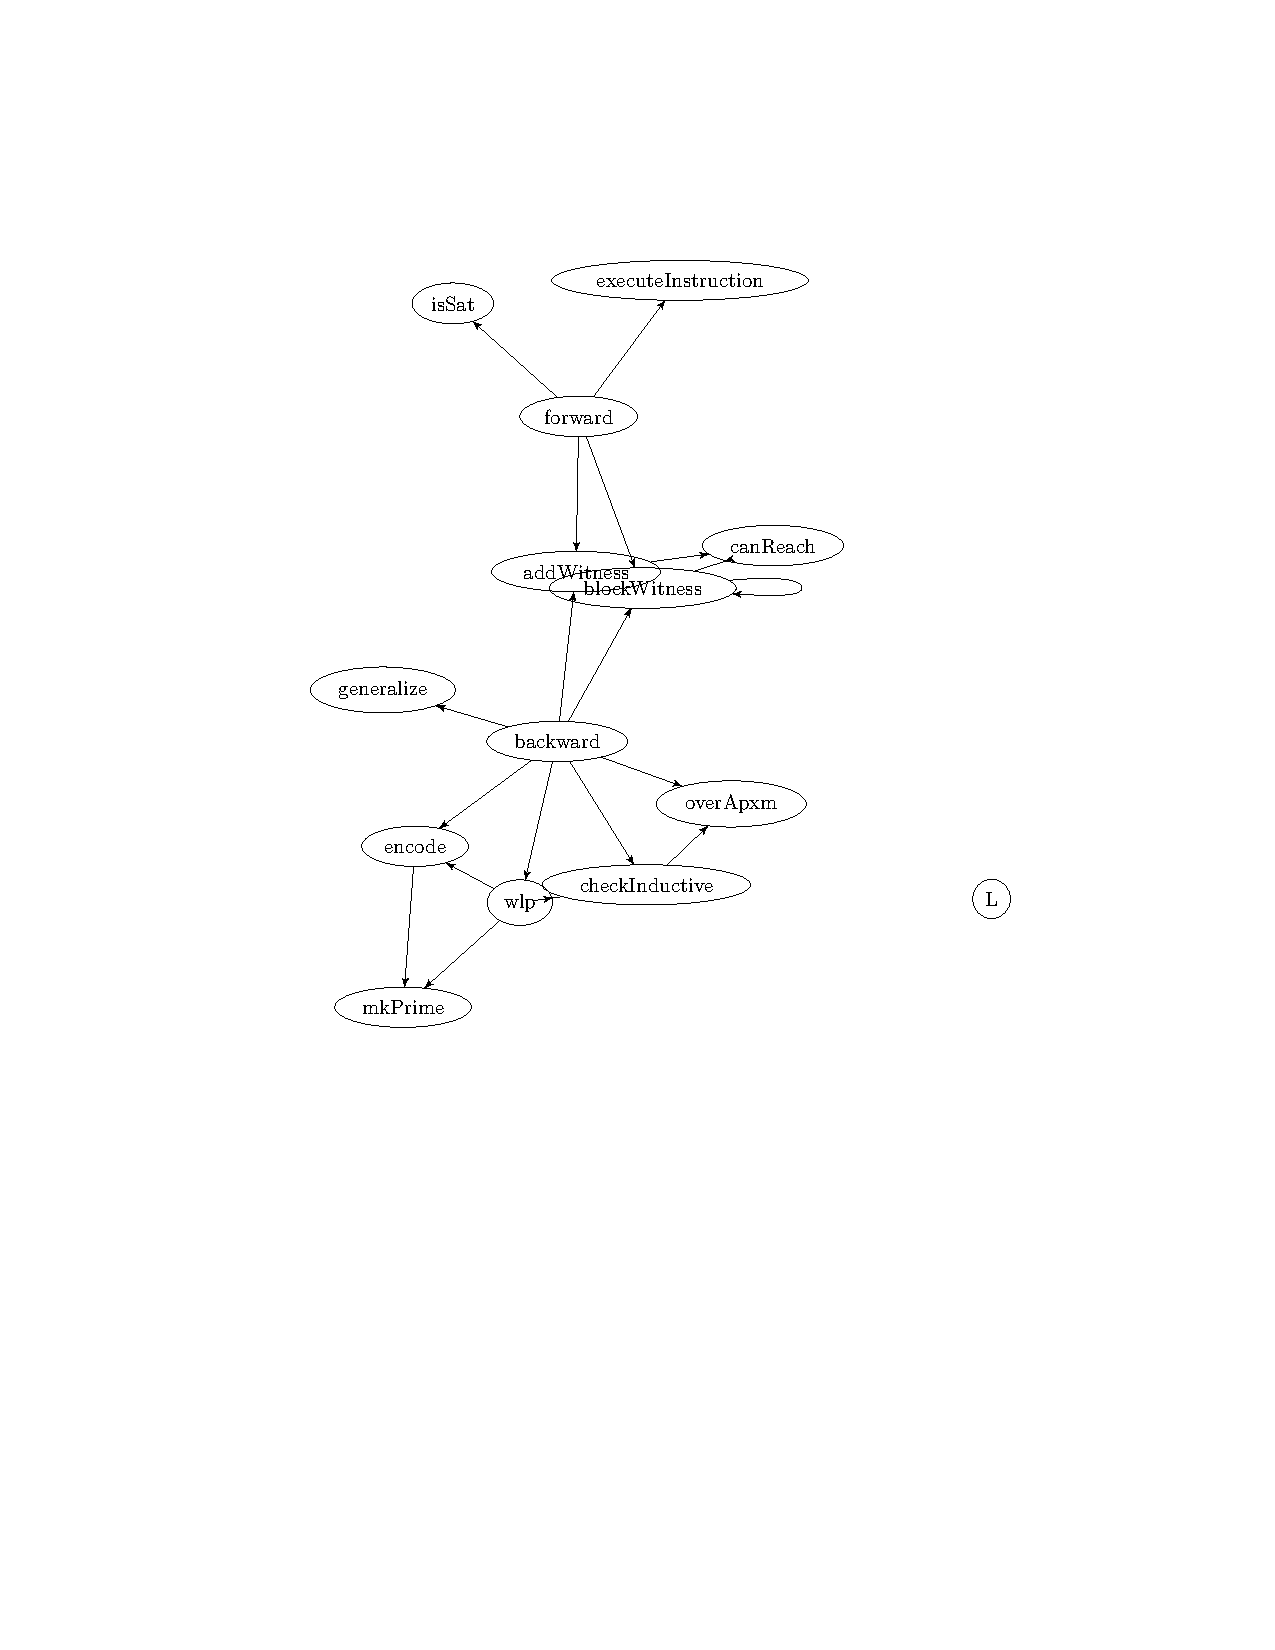
\includegraphics[height=15cm]{graph.pdf}
\end{frame}

\begin{frame}[fragile]
\begin{minted}{ocaml}
val propDirSymExec: locs:(loc set) -> program -> unit
(* возвращает хрен знает что
*)

val start: loc -> unit 
(* обновляет startState, Qf, T(loc) 
и много раз вызывает addWitness
*)
\end{minted}
\end{frame}

\begin{frame}[fragile]
\begin{minted}{ocaml}
type pob = { loc : loc; φ : formula; lvl : level }
type state = {
loc : loc; PC : formula; store : store;
loc0 : formula; lvl : level; pobs : Set<pob> }

\end{minted}
\end{frame}
\begin{frame}[fragile]
% TODO: почему pygmentize так подсвечивает юникод?

\begin{minipage}{0.49\linewidth}
\begin{minted}{ocaml}
curLvl : level

mainPobs : pob set
(* главные запросы *)
pobs : pob set

Qf : state set

Qb : (pob * state) set
\end{minted}
\end{minipage}\hspace{0cm}
\begin{minipage}{0.49\linewidth}
\begin{minted}{ocaml}
witnesses : pob -> state set 
blockedLocs : (pob, loc set) map
pobsLocs : loc set
T : loc -> state set
L : loc × level -> formula set
\end{minted}

\end{minipage}

\end{frame}

\begin{frame}[fragile]
\begin{minted}{ocaml}
val propDirSymExec: loc set -> program -> unit 
(* изменяет pobs, curLvl
  вызывает ChooseAction, forward, backward, start, nextLevel
*)

val forward: state -> unit 
(* обновляет Qf,T
    вызывает blockWitness 
*)

val backward: pob -> state -> program -> level -> unit 
(* обновляет Qb, lvl, принятый pob, child
    вызывает WLP, overApxm, addWitness, encode,
              checkInductive, generalize, answerYes
*)
\end{minted}
\end{frame}

\begin{frame}[fragile]
\begin{minted}{ocaml}
val answerYes: pob -> 'wtf
val answerNo: pob -> 'wtf
(* выдают финальный ответ, не реализованы,
  Должны смотреть на pob, с помощью child находит его детей (? или родителей) 
  и обрушать их во множествах pobs и mainPobs
 *)
val child: (pob, pob set) map 
(* Так себе описан *)

val canReach: loc -> loc -> locs -> bool 
(* проверяет наличие межпроцедурного пути в CFG от локации loc1 до loc2, 
не посещающего ни одну из локаций locs
*)
val checkInductive: level -> unit 
(* обновляет L
  вызывает WLP, overApxm
*)
\end{minted}
\end{frame}

\begin{frame}[fragile]
\begin{minted}{ocaml}
val addWitness: state -> pob -> unit
(* вызывет canReach
  обновляет s.pobs и witnesses[state]
*)

val blockWitness: state -> pob -> unit 
(* обновляет witnesses, blockedLocs
  вызывет blockWitness, canReach
*)
\end{minted}
\end{frame}

\begin{frame}[fragile]
\begin{minted}{ocaml}
val eL: loc -> level -> formula

\end{minted}
Сильно использует в себе функцию 
\begin{minted}{ocaml}
val over_apxm : loc -> lvl:level -> cur_lvl:level -> formula
\end{minted}


\begin{minted}{ocaml}
val encode: state -> formula
(* Использует mkPrime *)

val wlp: state -> formula -> formula
(* Использует encode & mkPrime *)

\end{minted}
\end{frame}


\begin{frame}[allowframebreaks]
\frametitle<presentation>{Ссылки}
\begin{thebibliography}{10}

  \bibitem{icfp2020}
    Staged Selective Parser Combinators
    \newblock {\em Jamie Willis \& Nicolas Wu \& Matthew Pickering}
    \newblock \url{https://doi.org/10.1145/3409002}

  \bibitem{berlin2020}
    Garnishing Parsec With Parsley: A Staged Selective Parser Combinator Library
    \newblock {\em Jamie Willis}
    \newblock \url{https://www.youtube.com/watch?v=tJcyY9L2z84}


  \bibitem{selective}
     Selective Applicative Functors
    \newblock {\em Andrey Mokhov \& Georgy Lukyanov \& Simon Marlow \& Jeremie Dimino}
    \newblock \url{https://doi.org/10.1145/3341694}
 
  \bibitem{cuts}
    Библиотека FastParse для Scala
    \newblock \href{https://webcache.googleusercontent.com/search?q=cache:WSoAEDqEOakJ:https://www.lihaoyi.com/fastparse/}{Documentation}
   
  \bibitem{trylookahead}
    Try vs. lookahead
    \newblock \url{https://stackoverflow.com/questions/20020350}
    
%  \bibitem{gerasimov}
%     Курс математической логики и теории вычислимости
%     \newblock {\em Герасимов А.С.}     
%     \newblock \href{https://www.mccme.ru/free-books/gerasimov-3ed-mccme.pdf}{PDF}
%
%  \bibitem{}
%    A Tutorial Introduction to the Lambda Calculus
%    \newblock {\em Ra\'ul Rojas}     
%    \newblock \href{https://www.inf.fu-berlin.de/lehre/WS03/alpi/lambda.pdf}{PDF}
%
%  \bibitem{sicp}
%    Structure and Interpretation of Computer Programs
%    \newblock {\em Abelson, Harold and Sussman, Gerald Jay and {with~Julie~Sussman}}     
%    \newblock \href{https://web.mit.edu/alexmv/6.037/sicp.pdf}{PDF}
%
%  \bibitem{olegSKI}
%    λ to SKI, Semantically (Declarative Pearl)
%    \newblock {\em Oleg Kiselyov}
%    \newblock \href{http://okmij.org/ftp/tagless-final/ski.pdf}{PDF}
    
\end{thebibliography}
 \end{frame}



\end{document}
